\chapter{Used Technologies}
\section{Development Process Tools}
\subsection{Version Control: GitHub}
GitHub is a web-based platform that uses Git for version control and collaboration on software projects.
It enables developers to collaborate in real-time. Thhey can track changes, manage issues, and review code.
It was released in 2008 and in 2018 it was acquired by Microsoft\cite{githubDefinition}.
Github is widely used in the software development industry and in has become standard practice to 
use GitHub for version control. 

\subsection{Software Development: Visual Studio Code and Visual Studio}
Visual Studio Code (VS Code) is a free lightweight code editor developed by Microsoft.
It supports a wide range of programming langueges and has a rich collection of extensiont that can be used to 
enchance its functionality.
It was very convinient to use a single code editor for multiple programming languages and frameworks.
To be more specific, I used Visual Studio Code for ESP32 programming, along with Platform IO, 
which is an open-source ecosystem for IoT development. VSCode was also used for the Angular web application 
development. The Raspberry Pi was programmed using Python, I used Visual Studio Code and for remote access
I used SSH.

Visual Studio is a more comprehensive integrated development environment (IDE) that provides advance features
for software development, such as debugging, profiling, and testing.
Visual Studio is also developed by Microsoft and it is widely used in the software development industry.
Since the PiIrrigate's web API was developed in .NET, I used Visual Studio for the API development.

\subsection{System Architecture: Draw.io}
Draw.io is a free online diagramming tool that allows users to create flowcharts, 
UML diagrams, network diagrams, and more. 
Other alternatives include Lucidchart, Microsoft Visio, and Gliffy. But I found that Draw.io is easy to use
and provides a wide range of templates and shapes that can be used to create diagrams.

\subsection{Iot Device Management: Azure IoT Hub}
Azure IoT Hub is a cloud-based service that enables secure and reliable 
communication between IoT devices and the cloud.
It provides a way to connect, monitor, and manage IoT devices at scale.
Azure IoT Hub is used in the PiIrrigate project to manage the
communication between the Raspberry Pi and the web API.

\section{Communication Technologies}
\subsection{LoRa Radio Communication}
LoRa is a wireless modulation technique derived from Chirp Spread Spectrum (CSS) technology.
LoRa modulated transmission is robust against disturbances and can be received across great distances.
It has become popular, as one of the most used standards for device interconnection, mainly because of its
low power consumption and long-range capabilities\cite{lora}. This technology was used in the PiIrrigate project
to enable the communication between the ESP32 nodes and the ESP32 gateway connected to the Raspberry Pi.

\subsection{MQTT Protocol}
MQTT (Message Queuing Telemetry Transport) is a 
an OASIS standard lightweight messaging protocol for the Internet of Things (IoT).
It is designed as an extremely lightweight publish/subscribe messaging transport that is ideal for connecting 
remote devices with a small code footprint and minimal network bandwidth. 
In the PiIrrigate project, MQTT is used to send data from the Raspberry Pi to IoTHub
and from the web API to the web application.

\subsection{HTTP Protocol}
HTTP is an application layer protocol for transmitting hypermedia documents, such as HTML.
It was designed for communication between web browsers and servers, 
but it can also be used for machine-to-machine communication.
In the PiIrrigate project, HTTP is used to send data from the web API to the web application\cite{http}.

\subsection{SignalR and WebSockets}
SignalR is an open-source library for ASP.NET that simplifies 
the process of adding real-time web functionality to applications.
It allows server-side code to push content to connected clients instantly as it becomes available.
SignalR uses WebSockets as its primary transport protocol, but it can also fall back to other techniques like
Server-Sent Events or Long Polling if WebSockets are not available.
In the PiIrrigate project, SignalR is used to provide real-time communication 
between the web API and the web application.

\section{Programming Languages and Frameworks}
\subsection{C\# and .NET}
C\# is a modern, object-oriented programming language developed by Microsoft.
It is widely used for developing Windows applications, web applications, and cloud services.
.NET is a free, open-source developer platform that provides a wide range of tools and libraries 
for building applications.
In the PiIrrigate project, C\# and .NET are used to develop the web API that manages the communication
between the Raspberry Pi and the web application, as well as to handle data storage in the PostgreSQL database.

\subsection{Entity Framework Core}
Entity Framework Core (EF Core) is an open-source, lightweight, extensible, and cross-platform version 
of the Entity Framework, which is an object-relational mapper (ORM) for .NET.
EF Core allows developers to work with databases using .NET objects, eliminating the need for 
most of the data access code that developers usually need to write.
In the PiIrrigate project, EF Core is used to interact with the PostgreSQL database,

\subsection{Python}
Python is a high-level, interpreted programming language known for its simplicity and readability.
It is widely used in various domains, including web development, data analysis, machine learning, and IoT.
In the PiIrrigate project, Python is used to develop the code that runs on the Raspberry Pi,
which is responsible for receiving data from the ESP32 nodes and sending it to the web API.

\subsection{Arduino C/C++}
Arduino C/C++ is a simplified version of C/C++ that is used to program Arduino 
boards and other microcontrollers.
It provides a set of libraries and functions that make it easy to interact with hardware components.
In the PiIrrigate project, Arduino C/C++ is used to program the ESP32 nodes that collect data from the sensors
and send it to the gateway using LoRa radio communication.

\subsection{Angular and TypeScript}
Angular is a platform and framework for building single-page client applications using HTML and TypeScript.
It is developed and maintained by Google and is widely used for building modern web applications.
In the PiIrrigate project, Angular is used to develop the web application that provides a user interface for
monitoring and controlling the irrigation system.

TypeScript is a superset of JavaScript that adds static typing and other features to the language.
It is designed for large-scale applications and provides better tooling and error checking compared to JavaScript.
JavaScript is a high-level, interpreted programming language that is widely used for building web applications.
It is primarly used for client-side scripting, but it can also be used for
 server-side development using Node.js.

\chapter{PiIrrigate System Overview}\label{section:overview}

\section{Overview}
The Internet of Things (IoT) is a new technology that allows devices to connect remotely to achieve smart
farming \cite{agriculture12101745}. The IoT has a wide range of applications in agriculture, and it has 
began to influence many other industries as well, such as healthcare, transportation, and manufacturing. 
This was done to improve the efficiency and productivity of these industries, 
as well as to reduce costs and improve the quality of products and services\cite{s19081833}.

The PiIrrigate smart irrigation system is build using a combination of hardware and software technologies.
It leverages both low-power edge devices and cloud-based infrastructure to provide real-time monitoring
and data collection, as well as remote control capabilities.
The core components and their roles in the system are as follows:
\begin{itemize}
  \item \textbf{ESP32 (LILYGO Meshtastic AXP2101 T-Beam V1.2 ESP32 LoRa)} \\
  The LILYGO Meshtastic AXP2101 T-Beam V1.2 ESP32 LoRa is a development board based on the ESP32 microcontroller, it is equipped with
  LoRa radio communication capabilities, Wifi, Bluetooth, GPS, and a battery management system.
  It is used to collect data from sensors and send it to the gateway using LoRa radio communication.

  \item \textbf{Raspberry Pi} \\
  Raspberry Pi is a small, affordable computer that can be used for a wide range of applications.
  The Raspberry Pi is the core of the PiIrrigate irrigation module, 
  it is responsible for receiving data from the ESP32 nodes and sending it to Azure IoT Hub.

  \item \textbf{Azure IoT Hub} \\
  Azure IoT Hub is a cloud-based service that enables secure and reliable communication 
  between IoT devices and the cloud.
  It manages the bidirectional communication between the Raspberry Pi and the web API.

  \item \textbf{Web API} \\
  The web API is developed in .NET and is responsible for receiving data from the Raspberry Pi,
  storing it in a PostgreSQL database, and providing a way to access the data.
  SignalR is used to provide real-time communication between the server and the client.
  It also provides a way to control the system manually and to add new nodes to the system.

  \item \textbf{PostgreSQL Database} \\
  PostgreSQL is a powerful, open-source relational database management system.
  It is used to store the data collected from the sensors and the schedules sent to the system. It also
  stores the user data and the configuration of the system. The database is hosted in Neon.

  \item \textbf{Web Application} \\
  The web applicaiton is developed using Angular and is responsible for displaying live, historical data
  and provide the user interface for controlling the system.
\end{itemize}

In the following sections, we will explore each of these components in more detail,
starting with the hardware components and then moving on to the software components.

\section{Hardware Components}
\subsection{Sensors}
The PiIrrigate system uses a variety of sensors to collect data from the environment.
The sensors used in the PiIrrigate system are:
\begin{itemize}
  \item \textbf{Soil Moisture Sensor} \\
  The soil moisture sensor is used to measure the moisture level in the soil. It is used to determine when to irrigate the plants.
  The sensor is connected to the ESP32 board and sends the data to the gateway using LoRa radio communication.

  \item \textbf{Temperature and Humidity Sensor} \\
  The temperature and humidity sensor is used to measure the temperature and humidity of the environment.
  It is used to determine the optimal conditions for plant growth and to adjust the irrigation schedule accordingly.

  \item \textbf{Rain Sensor} \\
  The rain sensor is used to detect rain and prevent irrigation during rainy weather. 
  It helps to conserve water and prevent over-irrigation.

  \item \textbf{Water Flow Sensor} \\
  The water flow sensor is used to measure the flow rate of water in the irrigation system.
  It is used to monitor the water consumption.

  \item \textbf{Water Temperature Sensor} \\
  The water temperature sensor is used to measure the temperature of the water in the irrigation system.
  It is used to ensure that the water temperature is within the optimal range for plant growth.


\end{itemize}
\subsection{ESP32 (LilyGo T-Beam)}

The T-Beam ESP32 LoRa Wireless Module is a compact development board thaht combines an ESP32 microcontroller,
LoRa transceiver (SX1278), GPS module, and a battery management system into a single unit. This board is ideal
for long-range, low-power IoT applications such as mesh networks, asset tracking, smart agriculture and environmental
monitoring. Besides this, it has a built-in OLED display. The communication range of the LoRa transceiver can reach up to 10 km in open areas.
\begin{figure}[H]
    \centering
    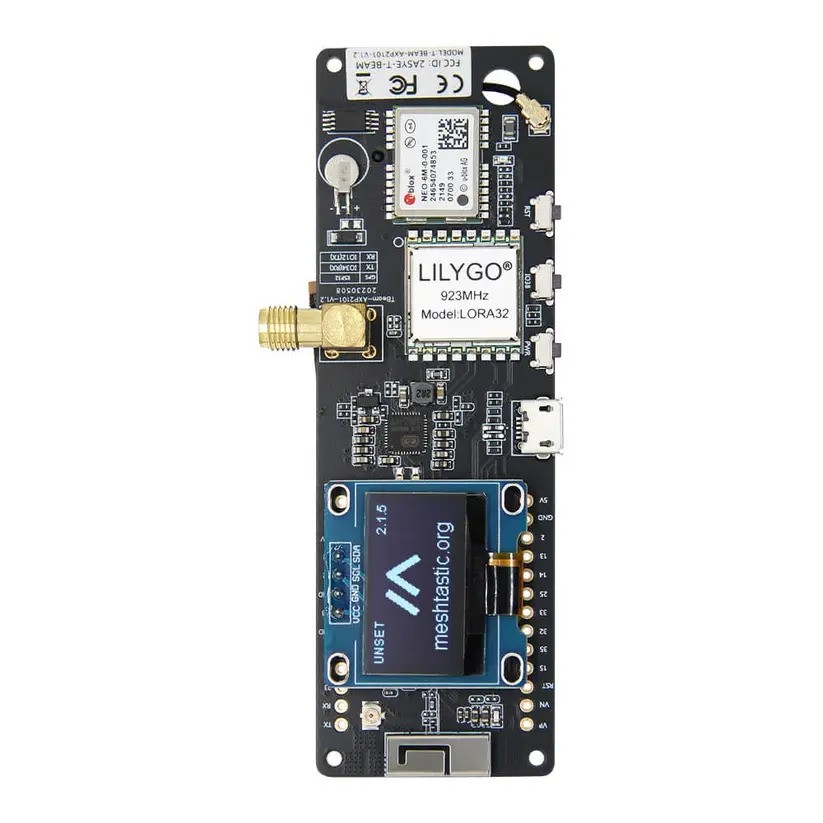
\includegraphics[width=0.8\textwidth]{images/esp32lora.jpg}
    \caption{ESP32 (LilyGo T-Beam) module used in PiIrrigate}
    \label{fig:esp32lora}
\end{figure}

\subsection{Raspberry Pi 4 Model B}
The Raspberry Pi 4 Model B is a small, affordable computer that can be used for a wide range of applications.
It is equipped with a quad-core ARM Cortex-A72 processor, up to 8GB of RAM, and supports dual-band Wi-Fi and Bluetooth.
The Raspberry Pi 4 Model B together with an ESP32LoRa is used in the PiIrrigate project as the gateway that receives data from the ESP32 nodes
and sends it to IoT Hub.
\begin{figure}[H]
    \centering
    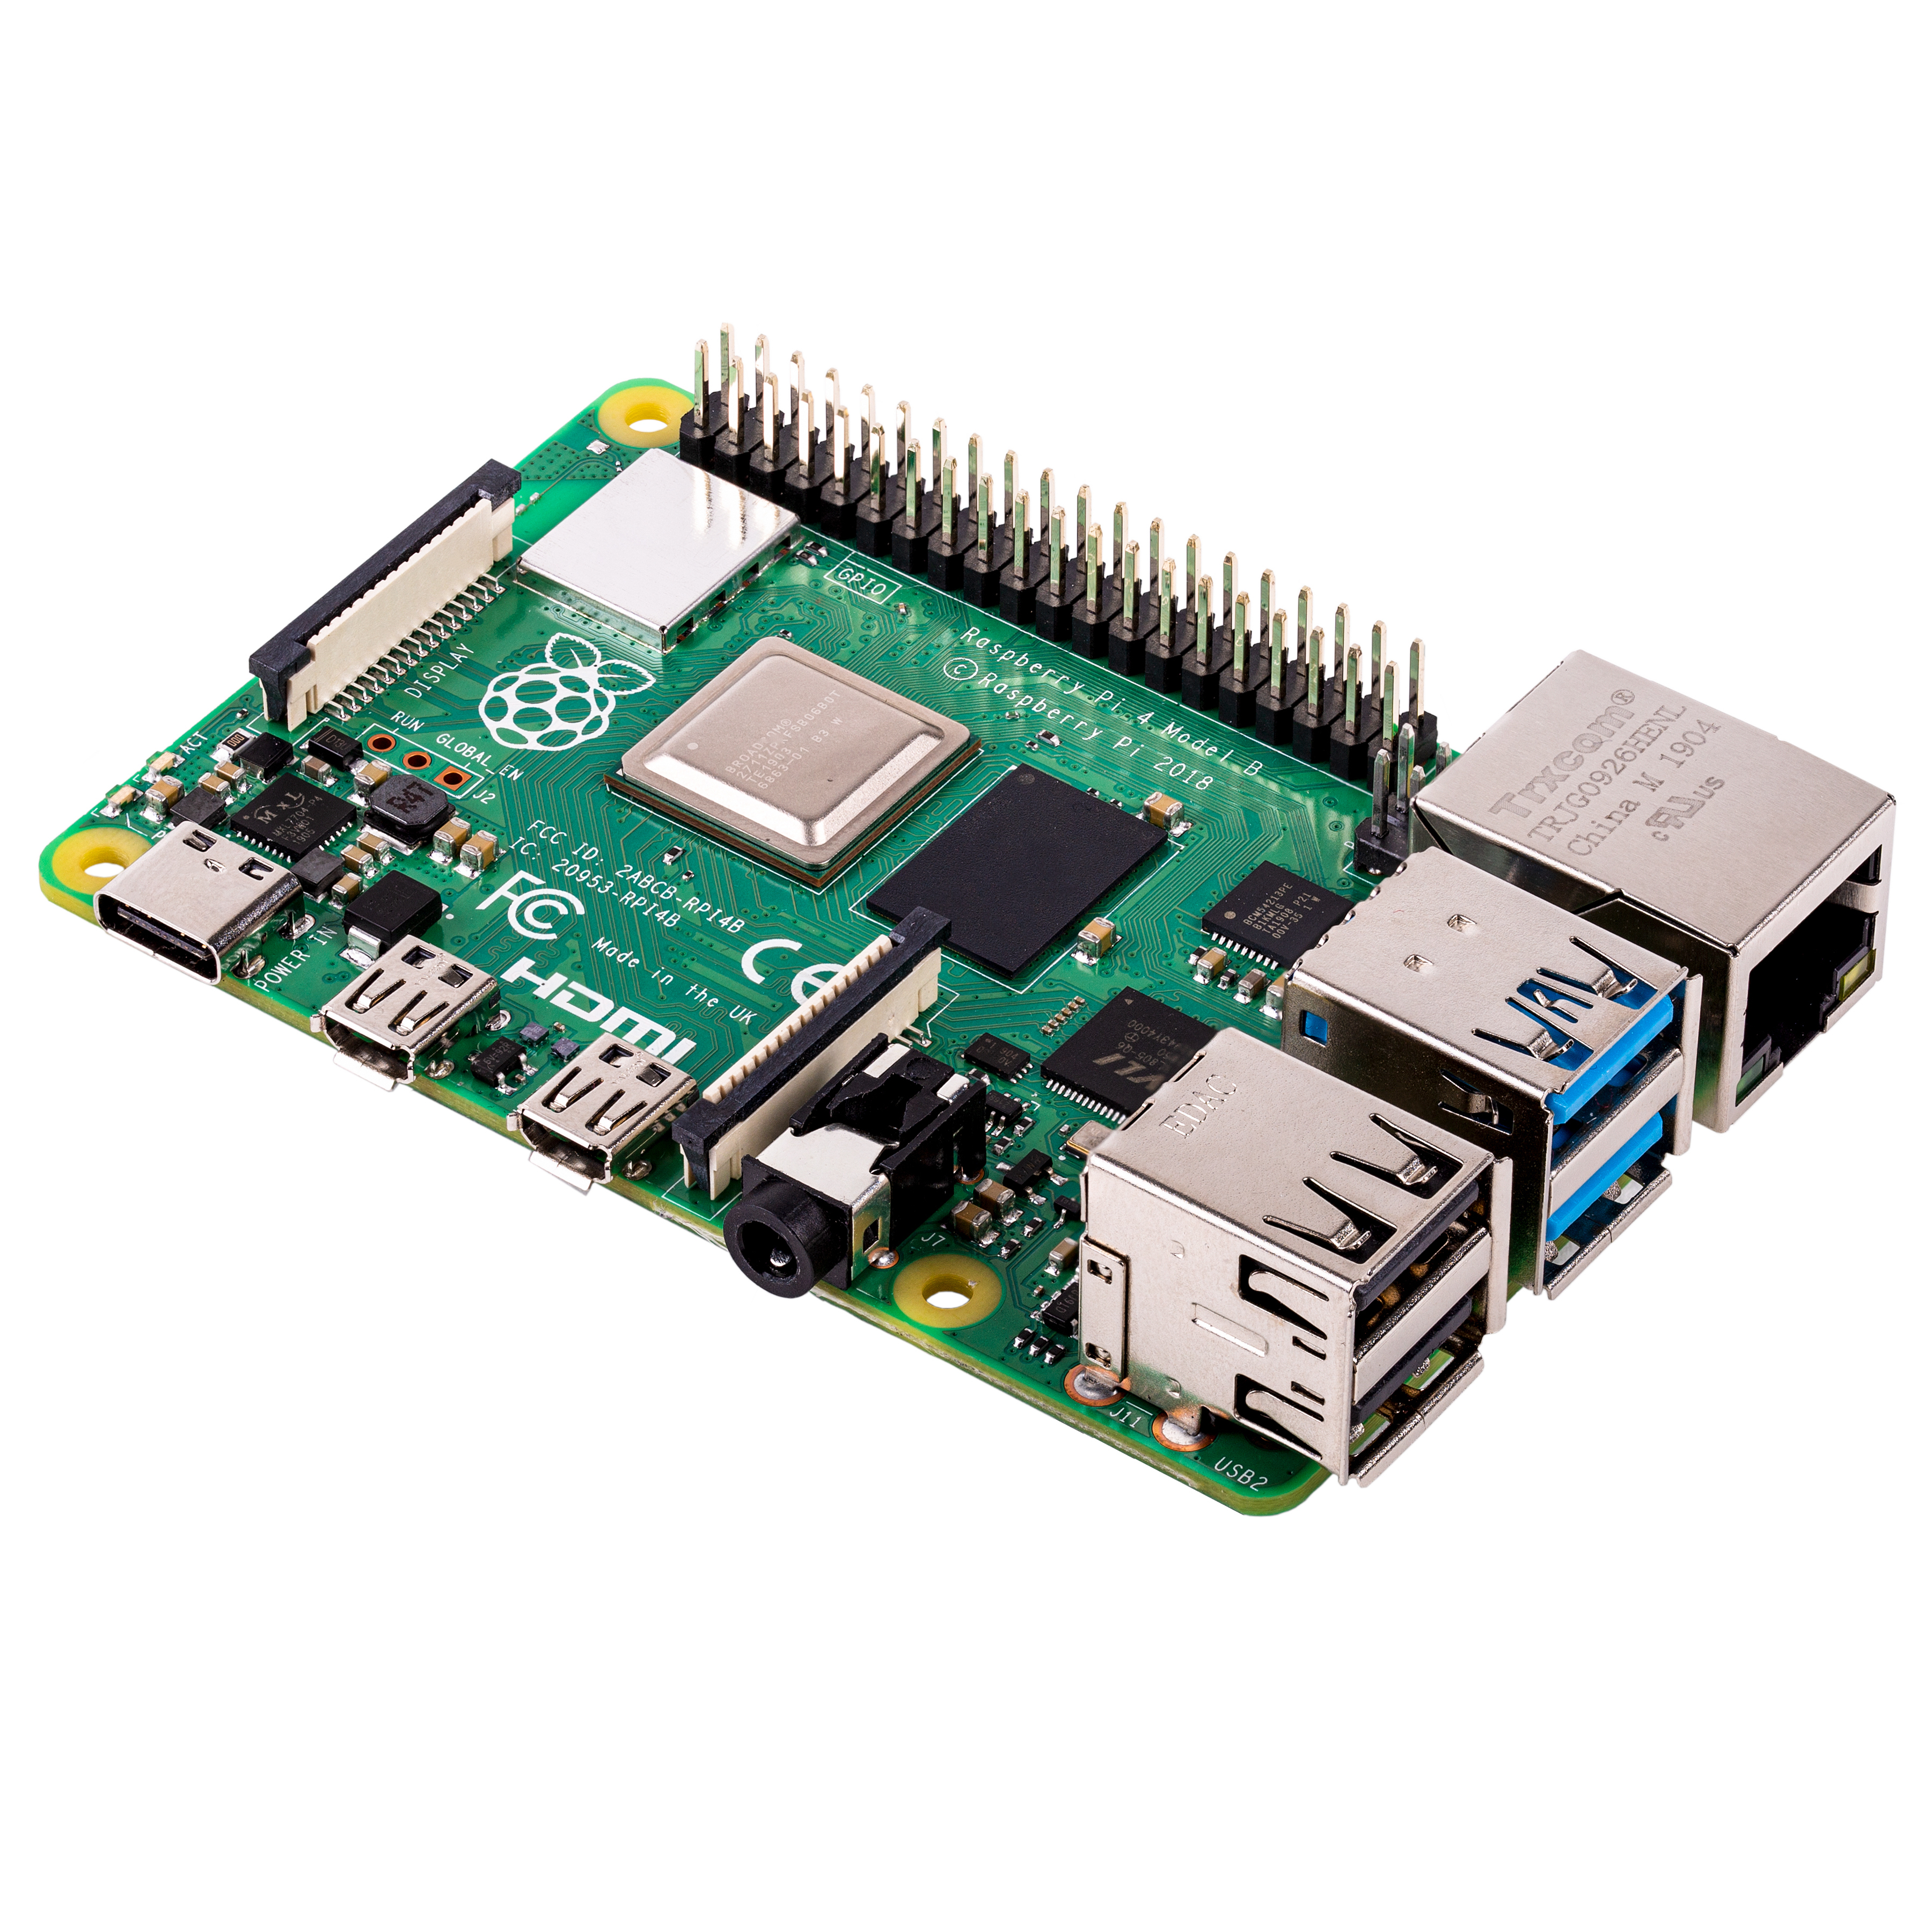
\includegraphics[width=0.8\textwidth]{images/raspberrypi.jpg}
    \caption{Raspberry Pi 4 Model B used in PiIrrigate}
    \label{fig:raspberrypi}
\end{figure}

\section{Data Flow}
The data flow in the PiIrrigate system is as follows:

\begin{enumerate}
  \item The ESP32 nodes collect data from the sensors and send it to the gateway using LoRa radio communication.
  \item The Raspberry Pi receives the data from the ESP32 nodes and sends it to Azure IoT Hub using MQTT protocol.
  \item The web API receives the data from Azure IoT Hub and stores it in the PostgreSQL database using Entity Framework Core. 
  \item The web application retrieves the data from the web API and displays it to the user in real-time using SignalR.
\end{enumerate}
\begin{figure}[H]
    \centering
    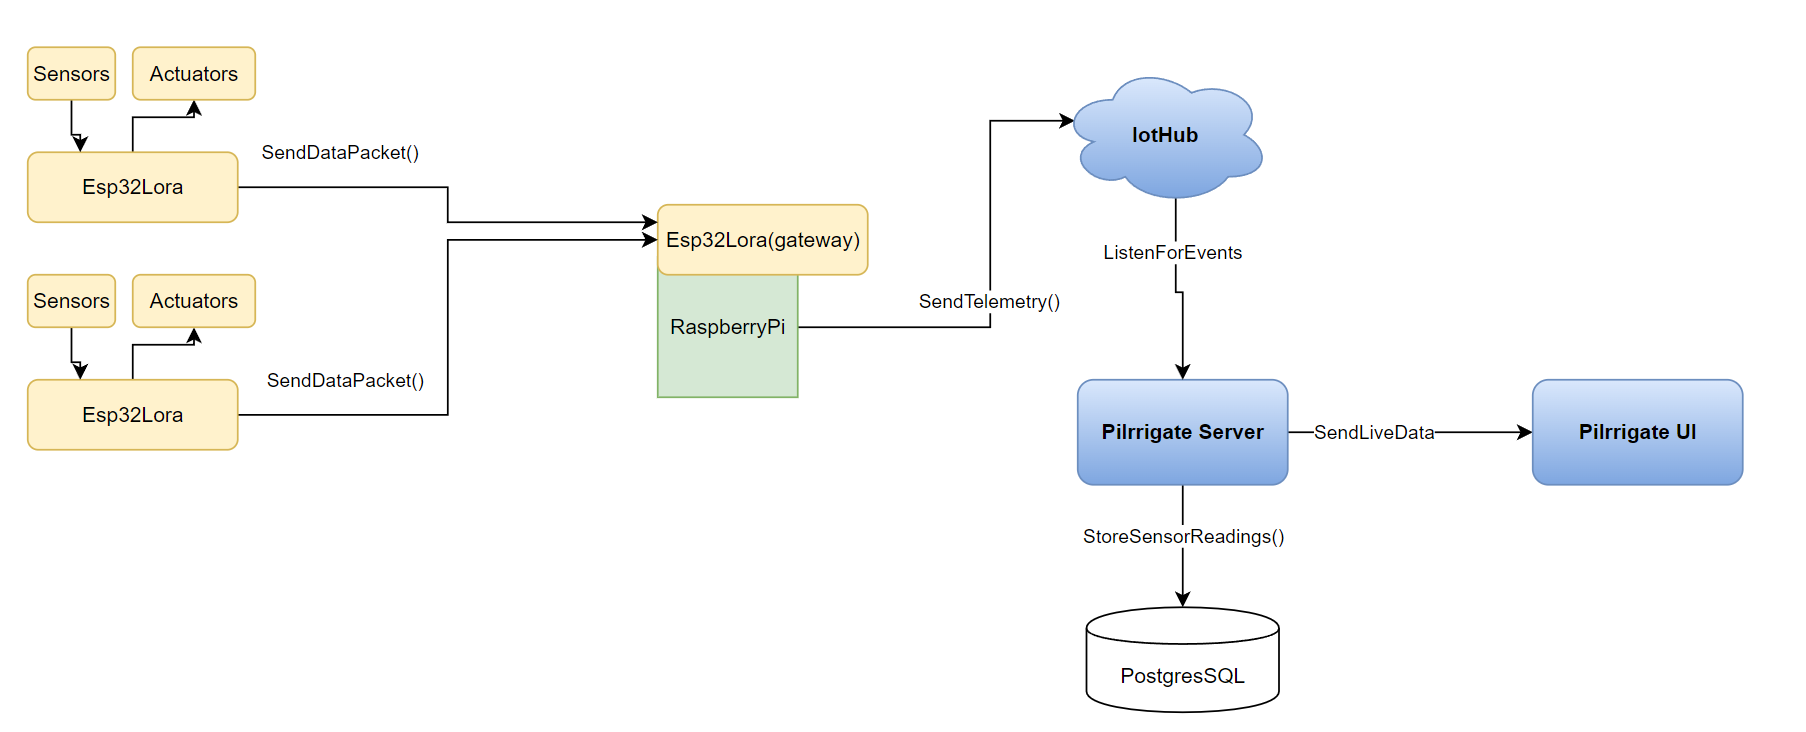
\includegraphics[width=0.8\textwidth]{images/system.png}
    \caption{PiIrrigate System overview}
    \label{fig:system-overview}
\end{figure}

\subsection{Data aquisition}
The data acquisition is done using the ESP32 nodes that collect data from the sensors.
For each sensor type, I created a specific library thath can be used to read the data from the sensor.
Temperature and humidity data is collected using a DHT11 sensor. The communication with the sensor is done using
1-wire digital interface. The communication is done in 3 steps\cite{1wire}:
\begin{enumerate}
  \item The microcontroller initiates communication by sending the start signal.
  The start signal is an 18\,ms LOW signal followed by a $20$--$40\,\mu$s HIGH signal.
  \item The sensor responds a fixed LOW and HIGH handshake pattern, indicating that it is ready to send data.
  Usually the acknowledgment is a $80\,\mu$s LOW signal followed by a $80\,\mu$s HIGH signal.
  \item After the handshake, the sensor sends a 40-bit data stream, which includes the humidity and temperature data.
  The bits are sent in a specific order: first the humidity data (16 bits), 
  then the temperature data (16 bits), 
  and finally a checksum (8 bits).
  Each bit is sent as a $50\,\mu$s LOW signal followed by a HIGH signal that lasts for either $26$--$28\,\mu$s (for a 0 bit) or $70\,\mu$s (for a 1 bit).
  In code, for each bit, the microcontroller waits for the LOW signal to start, 
  then waits for $30\,\mu$s then ig the signal is HIGH, the bit is a 1, otherwise it is a 0.
  The checksum is used to verify the integrity of the data received from the sensor.
\end{enumerate}

\begin{figure}[H]
    \centering
    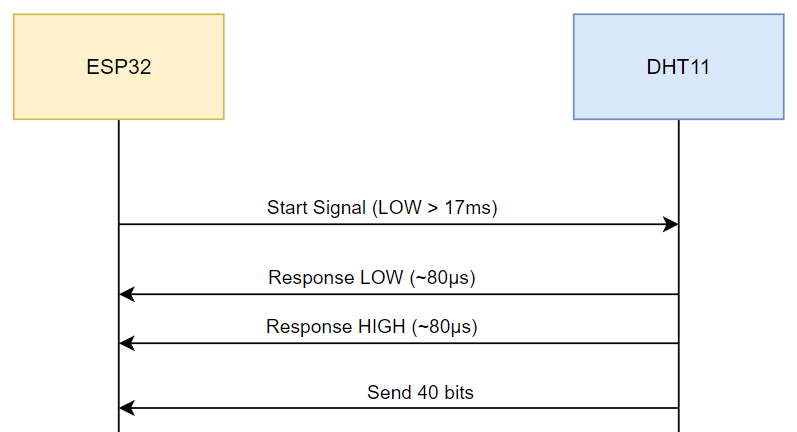
\includegraphics[width=0.8\textwidth]{images/dht-steps.png}
    \caption{Steps in data aquisition from DHT11 sensor}
    \label{fig:dht-steps}
\end{figure}

For the soil moisure data acquisition, I used a resistive soil moisture sensor. The principle of operation is based
on measuring the resistance of the soil. The sensor consists of two probes that are inserted into the soil.
When the soil is dry, the resistance between the probes is high, and when the soil is wet, the resistance is low\cite{s20020363}.
Then an ADC is used to measure the voltage across the probes, which is transofmerd into digital value. In this case, the
ADC is a 12-bit ADC, which means that the digital value can range from 0 to 4095.

For the rain sensor, I used a resistive rians sensor. The principle of operation is similar to the soil moisture sensor,
but it is designed to detect the presence of water on the sensor surface. 
When the sensor is dry, the resistance between the probes is high, and when it is wet, the resistance is low.

\begin{figure}[H]
    \centering
    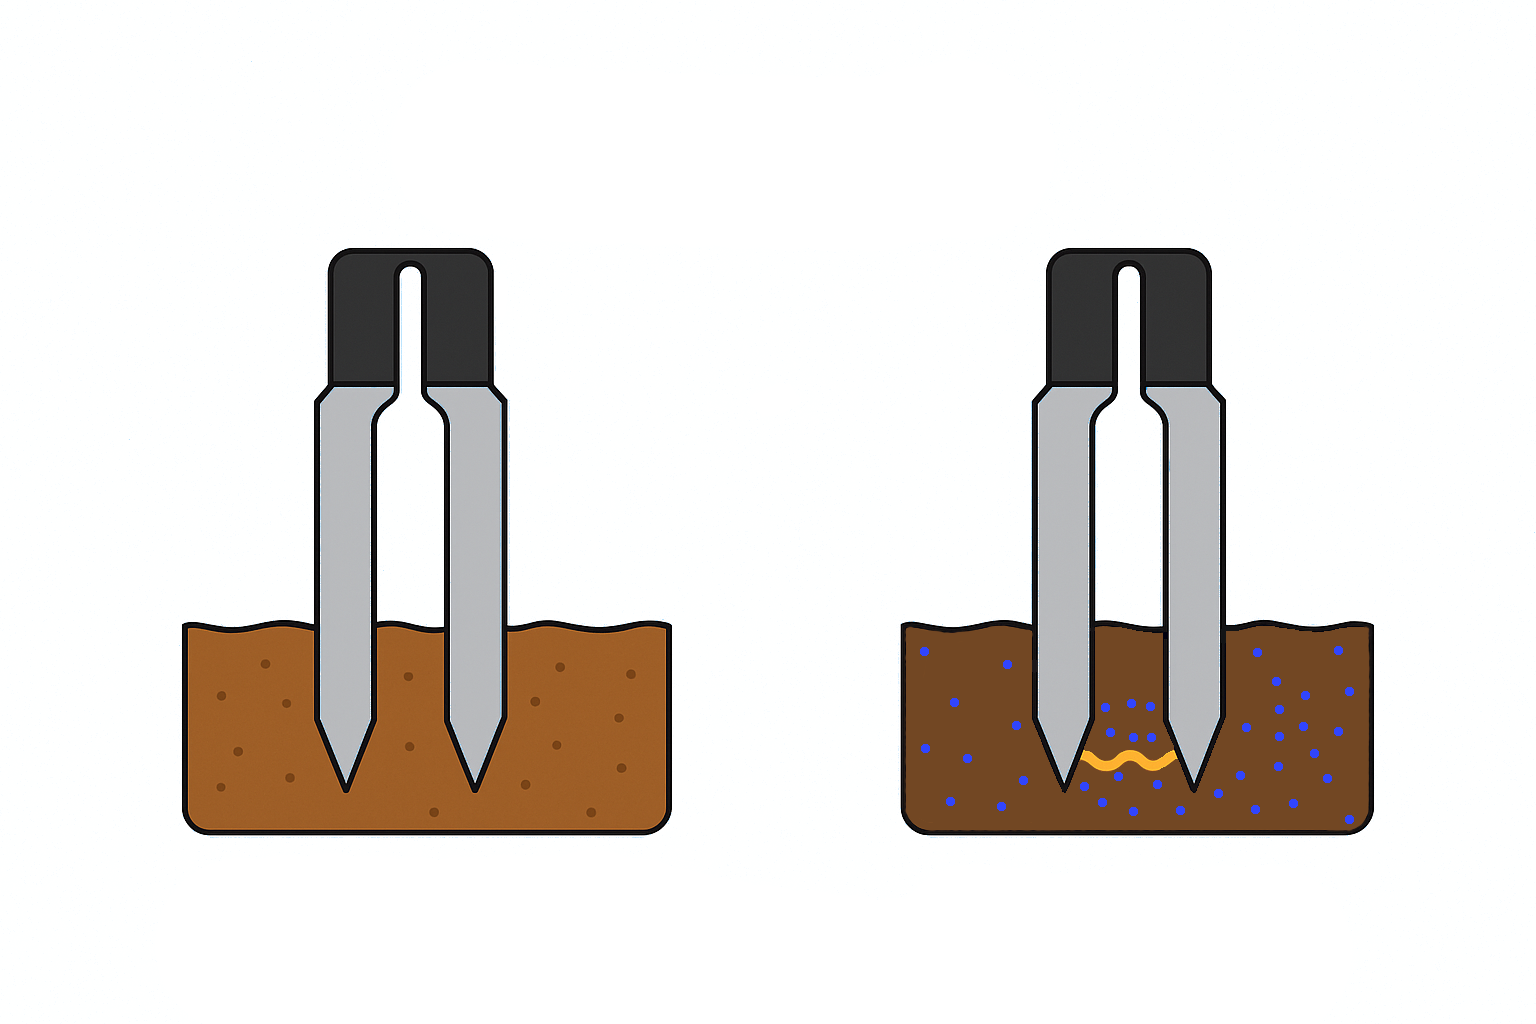
\includegraphics[width=0.7\textwidth]{images/moisture-sensor.png}
    \caption{Soil moisture sensor based on resistive principle}
    \label{fig:moisture-sensor}
\end{figure}

Since the water consumoption is a very important aspect in agriculture, 
I wanted to add a water flow sensor to the system. For the purpose of this project I used an 
YF-S201 water flow sensor, 
which is a low-cost sensor that can be used to measure the flow rate of water in a pipe.
The sensor consists of a plastic body with a 
turbine inside that rotates when water flows through it.
The rotation of the turbine generates a pulse signal that can be used to measure the 
flow rate of water.
The sensor has a maximum flow rate of 30 liters per minute and a minimum 
flow rate of 1 liter per minute.
The sensor has three wires: red (VCC), black (GND), and yellow (signal).
At each rotation of the tubine, the sesnsor generates a pulse signal on the signal wire.
The ESP32 counts the number of pulses in a given time interval 
(e.g., 1 second) to calculate the flow rate.
The flow rate can be calculated using the following formula:
\begin{equation}
    \text{Flow Rate} = \frac{\text{Number of Pulses} \times 60}{\text{Time Interval (seconds)}}
\end{equation}
\begin{figure}[H]
    \centering
    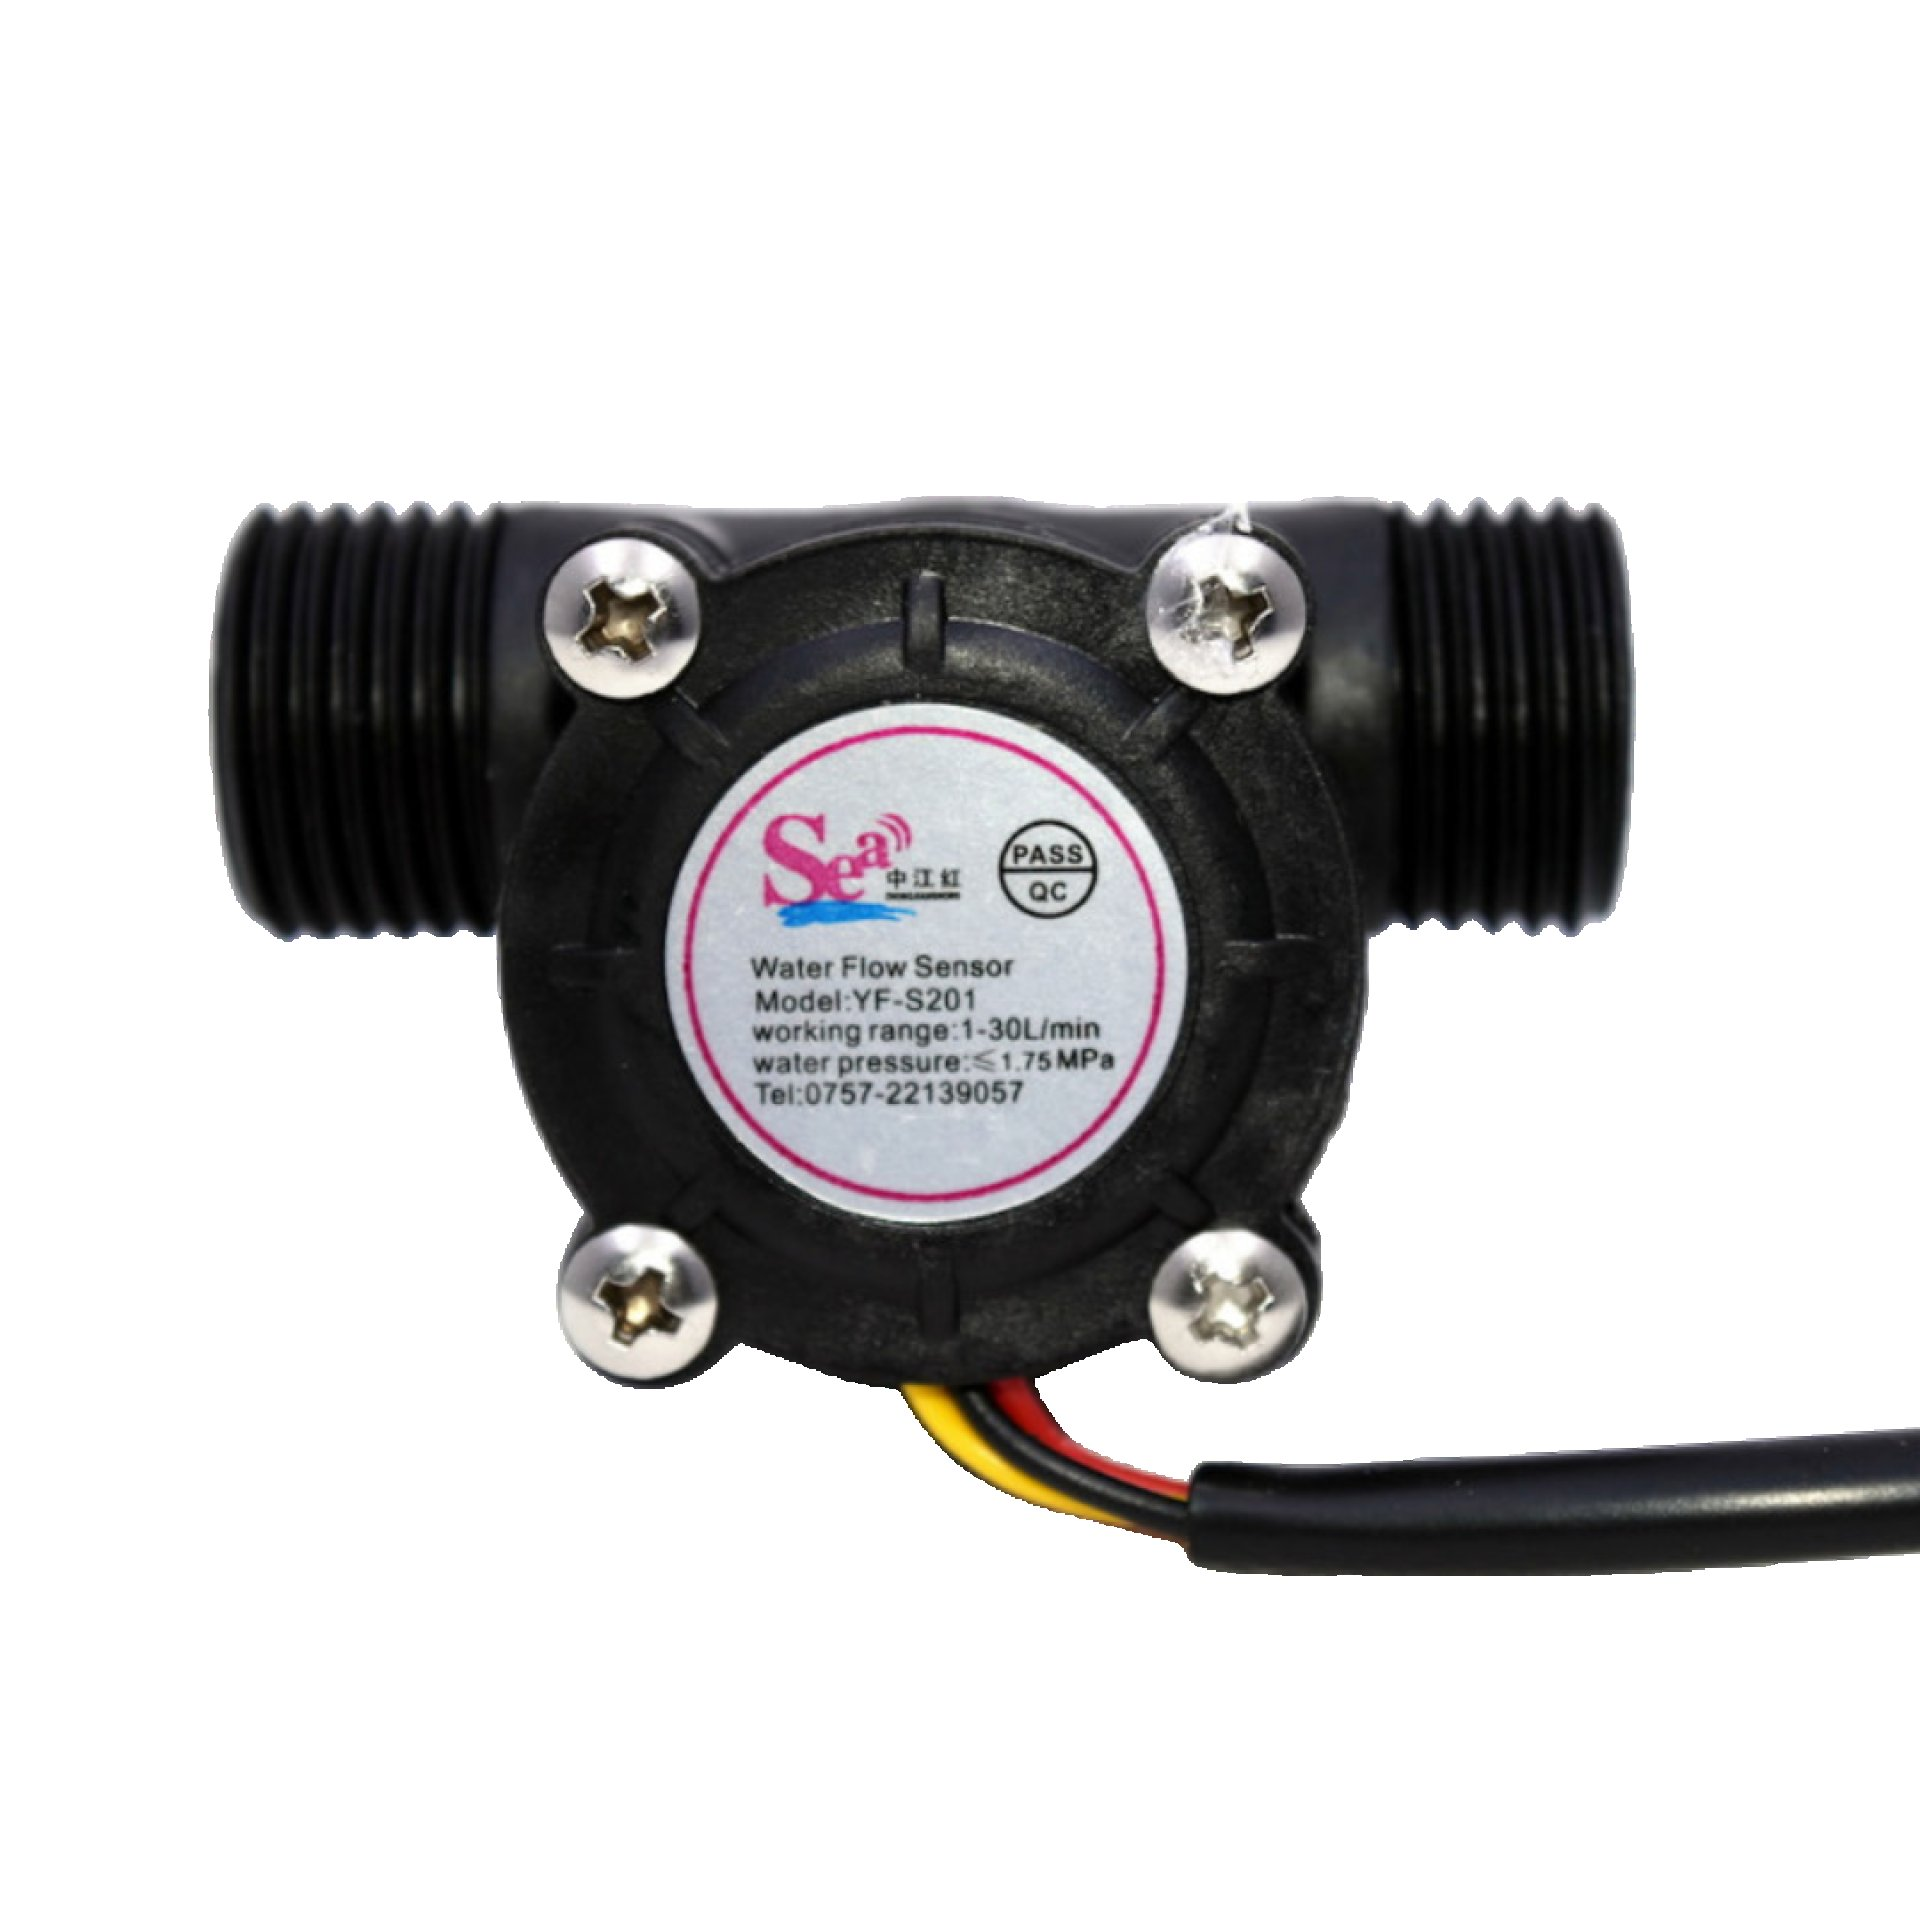
\includegraphics[width=0.5\textwidth]{images/water-flow.jpg}
    \caption{Water flow sensor used in PiIrrigate}
    \label{fig:water-flow-sensor}
\end{figure}

In my implementation, the water will be in a container, and during the irrigation process, 
the water will be deliverd to the plants using the gravity force. Because of this, I used
water temperature sensor to measure the temperature of the water in the container. 
The water temperature sensor is a DS18B20 sensor, 
which is a digital temperature sensor that can be used to measure the temperature of liquids.
The DS18B20 sensor uses the 1-wire digital interface to communicate with the ESP32.
The sensor can measure temperatures from -55°C to +125°C with an accuracy of ±0.5°C.

\begin{figure}[H]
    \centering
    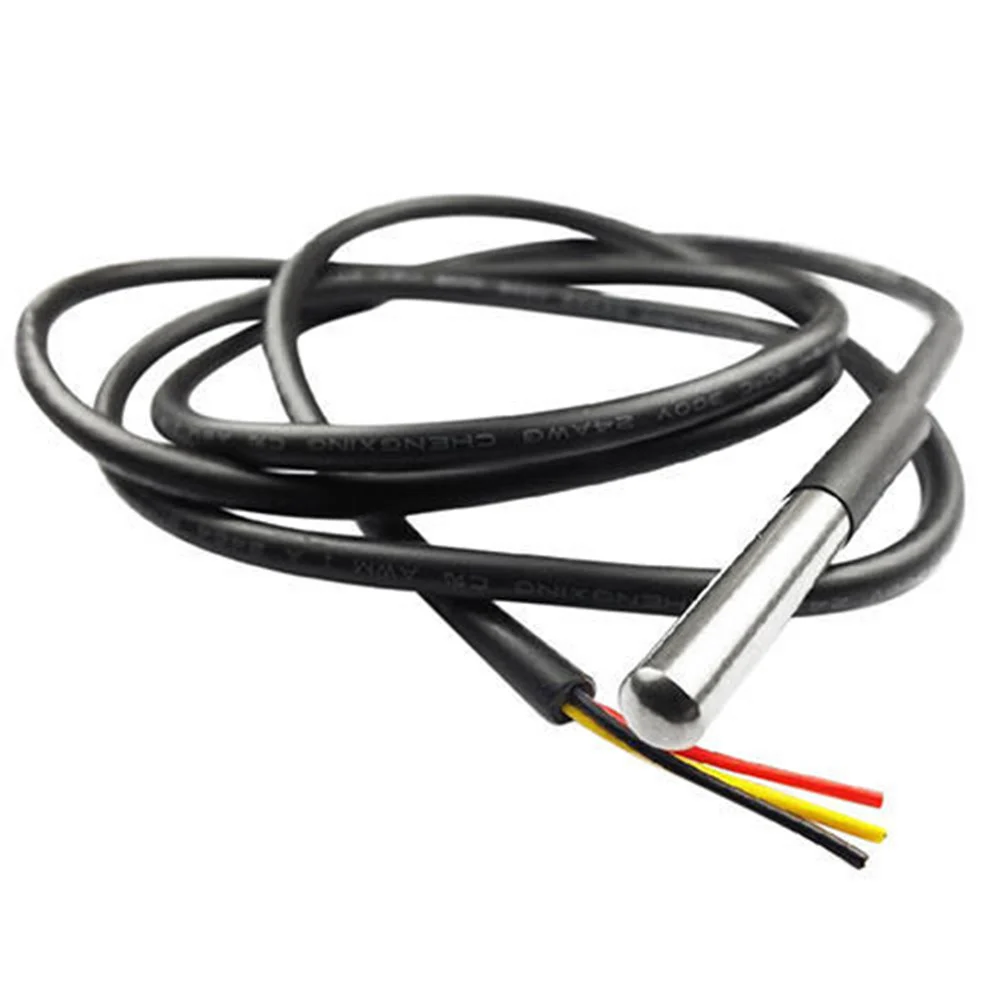
\includegraphics[width=0.5\textwidth]{images/water-temp.png}
    \caption{DS18B20 water temperature sensor used in PiIrrigate}
    \label{fig:ds18b20}
\end{figure}

Beside the sensors, I also used the GPS module of the T-Beam ESP32 board to 
ollect the GPS coordinates of the node. 
This can be useful for tracking the location of the node and for mapping the irrigation system.
The LILYGO Meshtastic AXP2101 T-Beam V1.2 ESP32 LoRa development board has a
NEO-6M GPS module, which is a high-performance GPS module that can provide accurate location data.

The GPIO25 pin of the ESP32 board is used to control the relay module that controls 
the electronic valve that opens and closes the water flow to the plants.
The relay module is a simple electronic switch that 
can be used to control high-voltage devices, such as water pumps or valves.

\subsection{ESP32 Pinout and Sensor Connections}
The ESP32 board has a variety of pins that can be used to connect the sensors and other components.
In the following diagram the connecttions between the ESP32 board and the sensors are shown.
\begin{figure}[H]
    \centering
    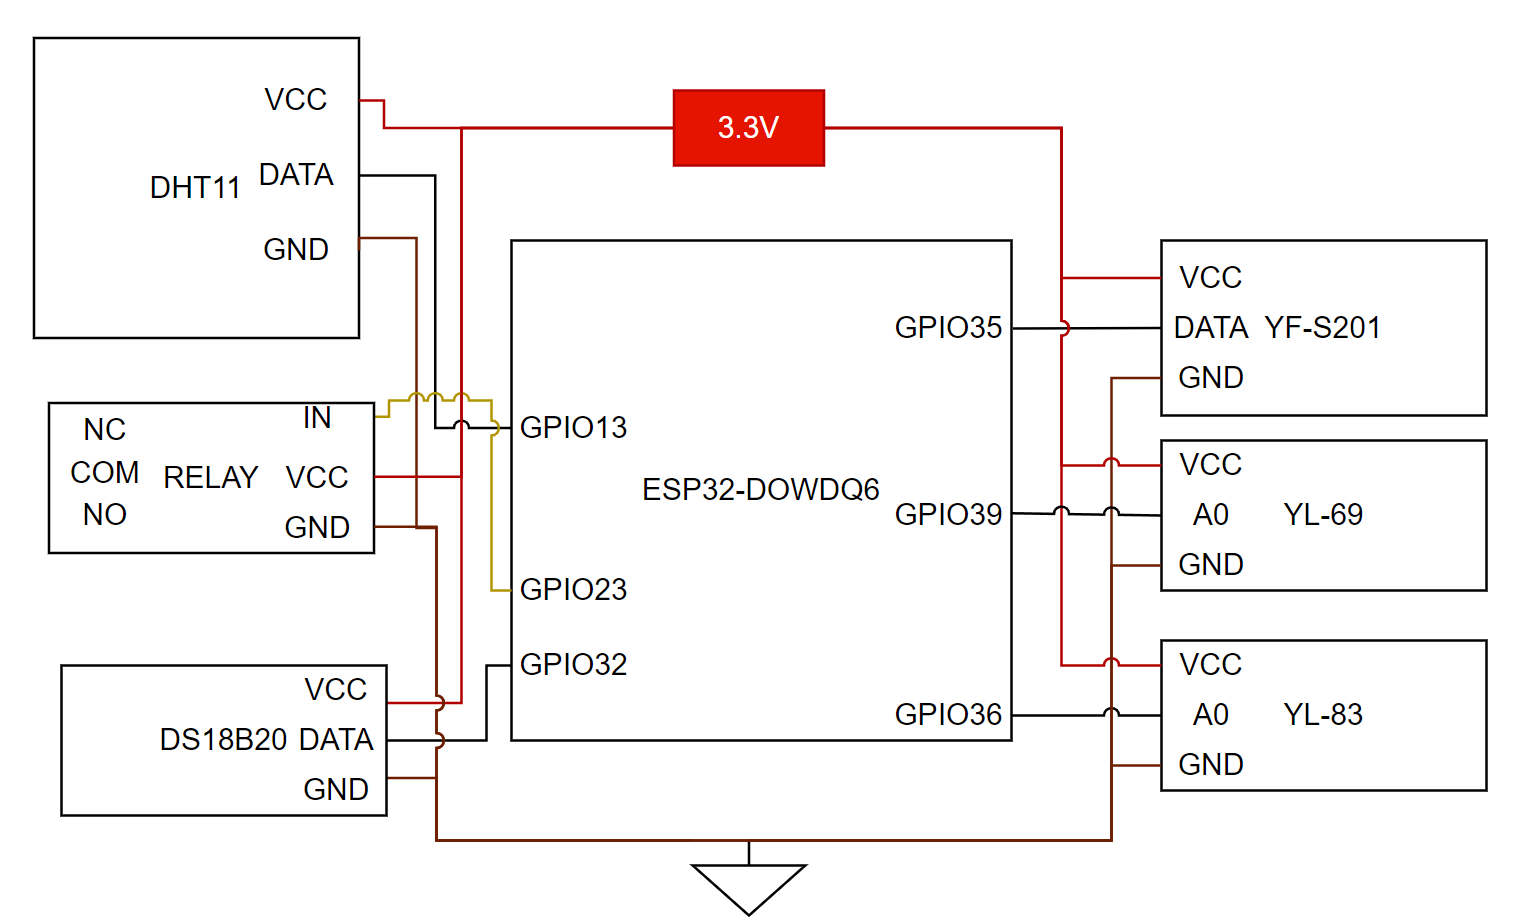
\includegraphics[width=0.8\textwidth]{images/esp-diagram.png}
    \caption{ESP32 pinout and connections}
    \label{fig:esp32-pinout}
\end{figure}

\subsection{LoRa Radio Communication}
LoRa (Long Range) is a wireless communication technology 
that is designed for long-range, low-power applications.
In this implementation, LoRa is used to send data from the nodes to the gateway.
The sensor reading has a period of 10 seconds, which is the default value, but this can be changed from the Web Application.
The data collected from the sensors is serialized into a sensor reading structure, 
which is then is included in a LoRa packet structure that will be 
binary serialized and sent over LoRa radio communication.

\begin{lstlisting}[language=C, caption={LoRa packet structure}]
struct LoRaPacket {
    int packetCount;      // Packet count for tracking
    SensorData sensorData; // Sensor data to be sent
    int stationMac[6]; // MAC address of the device
};
\end{lstlisting}

\begin{lstlisting}[language=C, caption={Sensor reading structure}]
struct SensorData {
    float temperature;
    float humidity;
    float soilMoisture;
    float rainLevel;
    float waterTemp;
    float totalWaterFlow;
    float longitude;
    float latitude;
};
\end{lstlisting}

All the values, except the totalWaterFlow, and the GPS coordinates, represent the raw
voltage values read from the sensors. I chose to sent the raw values, 
because they can be used to calculate the actual values in the web application.
Allowing a better flexibility in the future.

\subsection{Raspberry Pi and ESP32 Gateway}
The gateway ESP23 act like a proxy between the nodes and the Raspberry Pi.
It receives the LoRa packets from the nodes, and then it sends the data to 
the Raspberry Pi using Serial communnication by UART.

UART is an integrated cicuit that plays the most important role in serial communication.
It containts a parallel-to serial converter and a serial-to-parallel converter\cite{uderstandingUart}
\cite{laddha2013review}. The 
parrallel-to-serial converter ia used for data sent from Raspberry Pi to the ESP32,
and the serial-to-parallel converter is used for data sent from the ESP32 to the Raspberry Pi.
The UART frame format is as follows:
\begin{itemize}
    \item Start bit: 1 bit, always 0
    \item Data bits: 5 to 9 bits, usually 8 bits
    \item Parity bit: 1 bit, optional, used for error detection
    \item Stop bit: 1 or 2 bits, always 1
    \item Idle bit: 1 bit, always 1
\end{itemize}

After receiveing the data, the Raspberry Pi will deserialize 
the LoRa packet structure and will send the data to Azure IoT Hub 
using MQTT protocol. For handling the communication between the 
Raspberry Pi and the Azure IoT Hub, I used the Azure IoT SDK for Python.
I chose to use the Azure IoT SDK for Python, 
because it is easy to use and it provides a simple way to connect to 
Azure IoT Hub. Besides this, it also provides a way to manage the devices and 
to send and receive messages.

\section{Software Components}
\subsection{Azure IoT Hub}
Azure IoT Hub is a cloud based platform
that enables secure and reliable communication between IoT devices and cloud.
It is very user friendly, providing sdk for multiple programming languages, 
including Python, C\#, Java, and JavaScript. 
In Azure IoT Hub, 
devices are represented as \"IoT devices\", all data from a single Raspberry Pi is sent
to a single IoT device. In this paper, In this project, I will refere to the IoT device
as an \"Irrigation zone\", because it represents a single irrigation zone that is 
controlled by a single Raspberry Pi. And the term \"device\" will refer to the ESP32 nodes.

When the Raspberry Pi is started, it will automatically connect to the Azure IoT Hub,
and it will create a new IoT device if it does not exist. That irrigation zone will not be active
until the user will activate it from the web application. The user is able to
activate the irrigation zone using the code shown on RaspberryPi OLED display.
The code is a unique identifier for the irrigation zone and it is used only once.

As I said before, a single irrigation zone is represented as a single 
IoT device in Azure IoT Hub and the connected nodes. 
\begin{figure}[H]
    \centering
    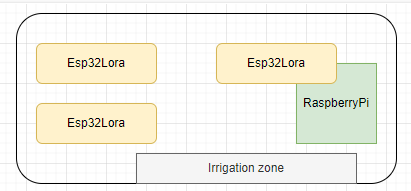
\includegraphics[width=0.8\textwidth]{images/irrigation-zone.png}
    \caption{Irrigaiton zone}
    \label{fig:irrigation-zone}
\end{figure}

\subsection{Zone Activation}

The activation process is done in the following steps:
\begin{enumerate}
    \item The user enters the code displayed on the Raspberry Pi OLED display in the web application.
    \item The web application sends the code to the web API.
    \item The web API verifies the code and activates the irrigation zone.
    \item The web API sends a message to the Iot Device to activate the irrigation zone.
    \item The Raspberry Pi receives the message from Azure IoT Hub and activates the irrigation zone.
    \item The Raspberry Pi sends a message to the ESP32 nodes to start collecting data from the sensors.
\end{enumerate}

\begin{figure}[H]
    \centering
    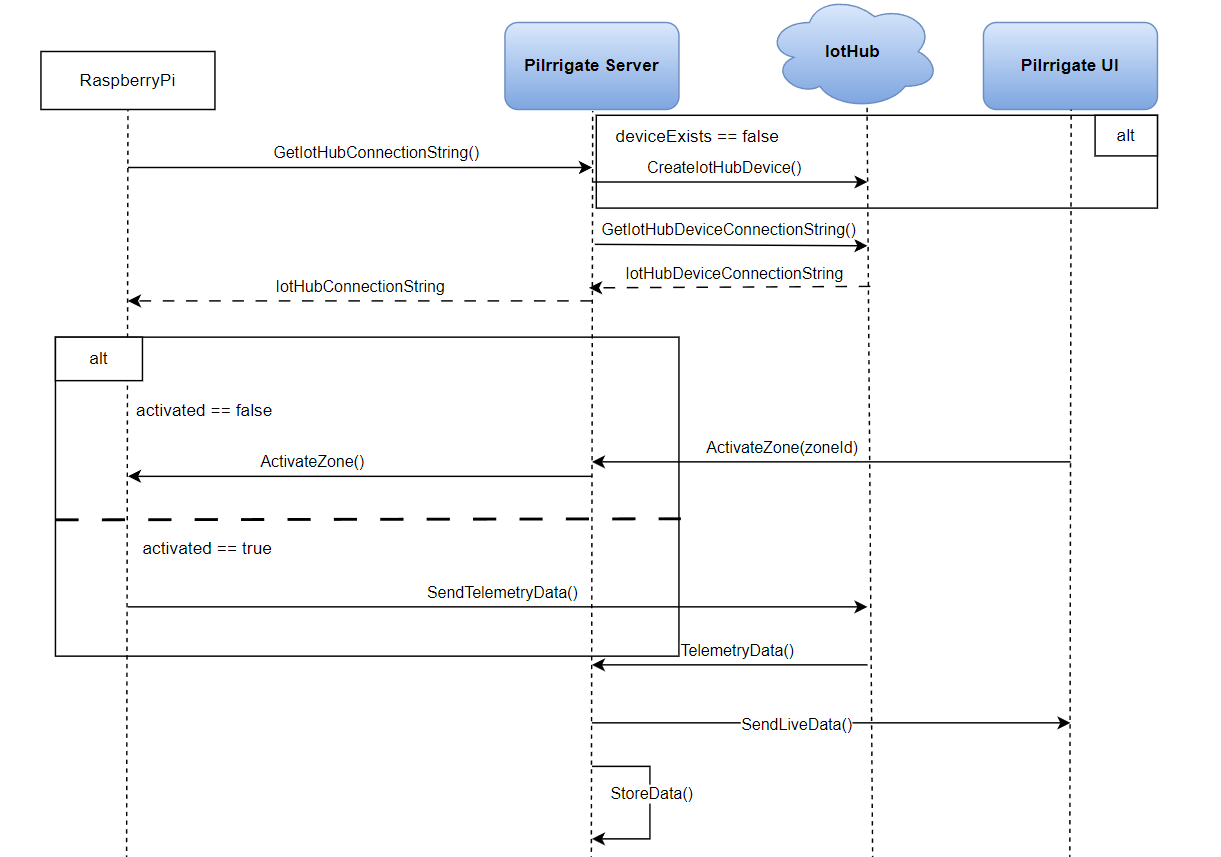
\includegraphics[width=0.9\textwidth]{images/activation.png}
    \caption{Zone activation process}
    \label{fig:zone-activation}
\end{figure}

\subsection{Web API}
The web API is developed in \.NET ans it is responsible
for user management, data storage, and communication with the IoT Hub.
It uses Entity Framework Core to interact with the 
PostgreSQL database and SignalR to provide real-time communication.
It uses the controller pattern to handle the HTTP requests. 
I created a controller for each resource in the system,
such as users, zones, data, devices, schedules and cloud to device messages.

\subsubsection{Zone Controller}
Since the first step in the activation process is to verify the code enterede by the
user, I will start describing the zone controller.
Using this controller, the user can create a zone, activate a zone, get the IoT Device connection string, retrieve
all zonees, get a zone by id, and delete a zone. For the database interaction, I created
a zone repository that implements the IZoneRepository interface.
\begin{lstlisting}[caption={Zone Repository interface}]
public interface IZoneRepository
{
    public Task<bool> CreateZone(Zone zone);
    public Task<bool> UpdateZone(Guid Id, string Name, Guid userId);
    public Task<bool> DeleteZone(Guid Id);
    public Task<Zone> GetZoneById(Guid Id);
    public Task<Zone> GetZoneByName(string name);
    public Task<IEnumerable<Zone>> GetAllByUserId(Guid Id);
}
\end{lstlisting}

The controller is also using the IoTDeviceManager service to manage the
IoT devices in Azure IoT Hub, which implement the IioTDeviceManager interface and 
is repsonsible for creating, deleting, and checking the existence of IoT devices.

\begin{lstlisting}[caption={IoT Device manager interface}]
public interface IiotDeviceManager
{
    public Task<bool> CreateIotDevice(string zoneId);
    public Task<string> GetDeviceConnectionString(string zoneId);
    public Task<bool> DeviceExists(string zoneId);
    public Task<bool> DeleteIotDevice(string zoneId);
}
\end{lstlisting}

\subsubsection{Data Controller}
The data controller is used to retrieve data from the PostgreSQL database.
It provides endpoints for:
\begin{itemize}
    \item Get all data for a zone, including the data for all devices in that zone.
    \item Get data for a certain period of time.
    \item Get all data foor a device.
    \item Get data for a device for a certain period of time.
\end{itemize}

The data controller will use the IDataService for all the logic related to data retrieval.
For the DataService, all the database interaction is done within that service.

\subsubsection{Device Controller}
The device controller is used to manage the devices in the system.
It provides endpoints for:
\begin{itemize}
    \item Get all devices for a zone.
    \item Get all devices for a user.
    \item Get a device by id.
    \item Get a device by MAC address.
    \item Register a new device.
\end{itemize}
\subsubsection{User Controller}
As the user needs to be authenticated to access the web API,
I created a user controller that handles user registration and login.

\begin{lstlisting}[caption={User Service interface}]
public interface IUserService
{
    Task<UserDto> GetUserByIdAsync(Guid userId);
    Task<IEnumerable<UserDto>> GetAllUsersAsync();
    Task<bool> UpdateUserProfileAsync(Guid userId, UpdateProfileRequest request);
    Task<bool> ChangeUserRoleAsync(Guid userId, string newRole);
    Task<AuthResult> RegisterUser(RegisterRequest register);
    Task<AuthResult> LoginUser(LoginRequest request);
}
\end{lstlisting}

For accessing the user data, UserRepository is used, which implements the IUserRepository interface.
The authorization is done using JWT tokens, 
which are generated when the user logs in. To handle all the logic related to 
JWT tokens, I created a JWT service that implements the IJwtService interface.
Besides IUserRespository, and IJwtService, the UserService is also using
IPasswordHasher to hash the user passwords. This provides abstraction
for hashing and verifying passwords, 
allowing for easy integration with different hashing algorithms. For the moment,
the implementation uses SHA256 hashing algorithm, 
but it can be easily changed to any other algorithm. In the future, I plan to replace
this with Microsoft.AspNetCore.Identity, 
which provides a more secure and flexible way to handle user 
authentication and authorization and it is widely used in the \.NET community.

\begin{lstlisting}[caption={User Repository interface}]
public interface IUserRepository
{
    Task<User> GetByIdAsync(Guid id);
    Task<User> GetByEmailAsync(string email);
    Task<IEnumerable<User>> GetAllAsync();
    Task<bool> CreateAsync(User user);
    Task<bool> UpdateAsync(User user);
    Task<bool> DeleteAsync(Guid id);
}
\end{lstlisting}

\begin{lstlisting}[caption={JWT Service interface}]
public interface IJwtService
{
    string GenerateJwtToken(User user);
    bool ValidateToken(string token);
}
\end{lstlisting}

\begin{lstlisting}[caption={Password Hasher interface}]
public interface IPasswordHasher
{
    string HashPassword(User user, string password);
    bool VerifyPassword(User user,string hashedPassword, string providedPassword);
}
\end{lstlisting}

\subsubsection{Registration Flow}
The registration flow is as follows:
\begin{enumerate}
    \item The user fills the registration form in the web application.
    \item The web application sends the request to the web API. More sdpecifically, 
    it sends a POST request to the register endpoint of the user controller. The controller
    receives the request as an object of type RegisterRequest.
    \item The request is being validated by the web API.
    \item If the request is valid, the web API creates a new user in the database
    \item The web API generates a JWT token and it sends back an object of type AuthResult.
    \item The web application receives the AuthResult object and stores the JWT token in the local storage.
\end{enumerate}

The registration flow is shown in the figure below.
\begin{figure}[H]
    \centering
    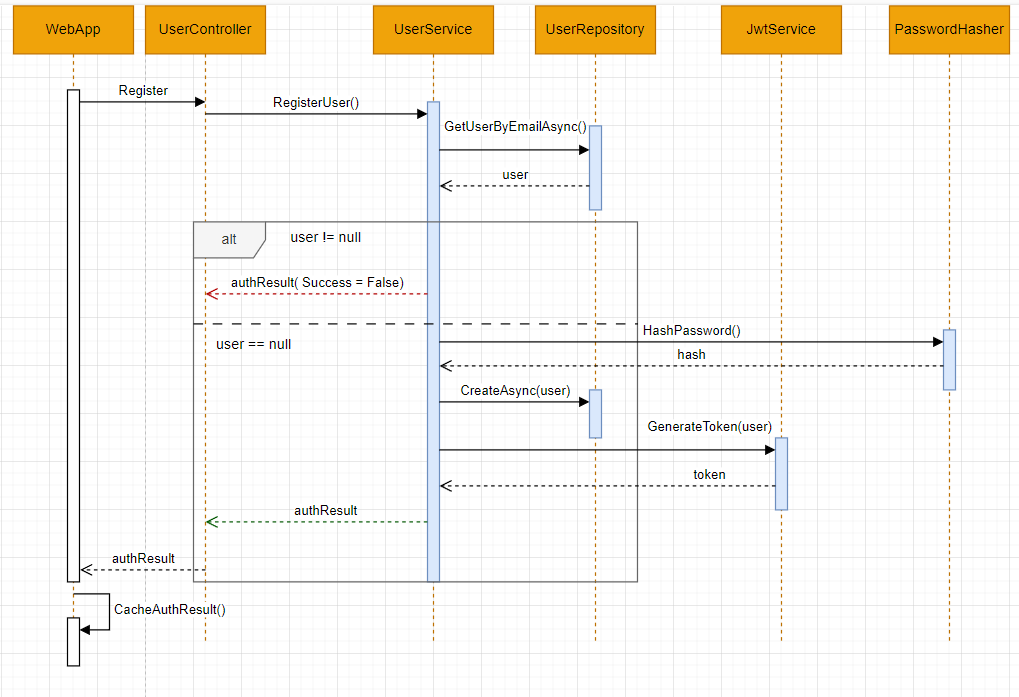
\includegraphics[width=0.9\textwidth]{images/registration-flow.png}
    \caption{Registration flow}
    \label{fig:registration-flow}
\end{figure}

The AuthResult object and the RegisterRequest object are defined as follows:
\begin{figure}[H]
    \centering
    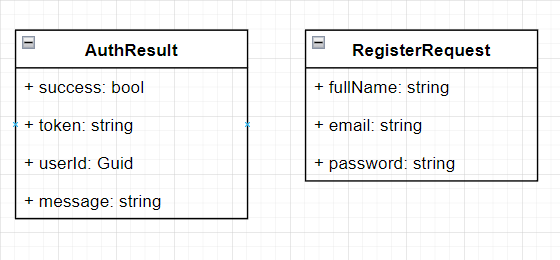
\includegraphics[width=0.8\textwidth]{images/auth-request.png}
    \caption{AuthResult and RegisterRequest objects}
    \label{fig:auth-result}
\end{figure}

\subsection{Login Flow}
The login flow is similar to the registration flow, but it does not create a new user.
The login flow is as follows:
\begin{enumerate}
    \item The user fills the login form in the web application.
    \item The web application sends a POST request to the login endpoint of the user controller. The controller
    receives the request as an object of type LoginRequest.
    \item The request is being validated by the web API.
    \item If the request is valid, the web API checks if the user exists in the database.
    \item If the user exists, the web API verifies the password and generates a JWT token.
    \item The web API sends back an object of type AuthResult.
    \item The web application receives the AuthResult object and stores the JWT token in the local storage.
\end{enumerate}

The login flow is shown in the figure below.
\begin{figure}[H]
    \centering
    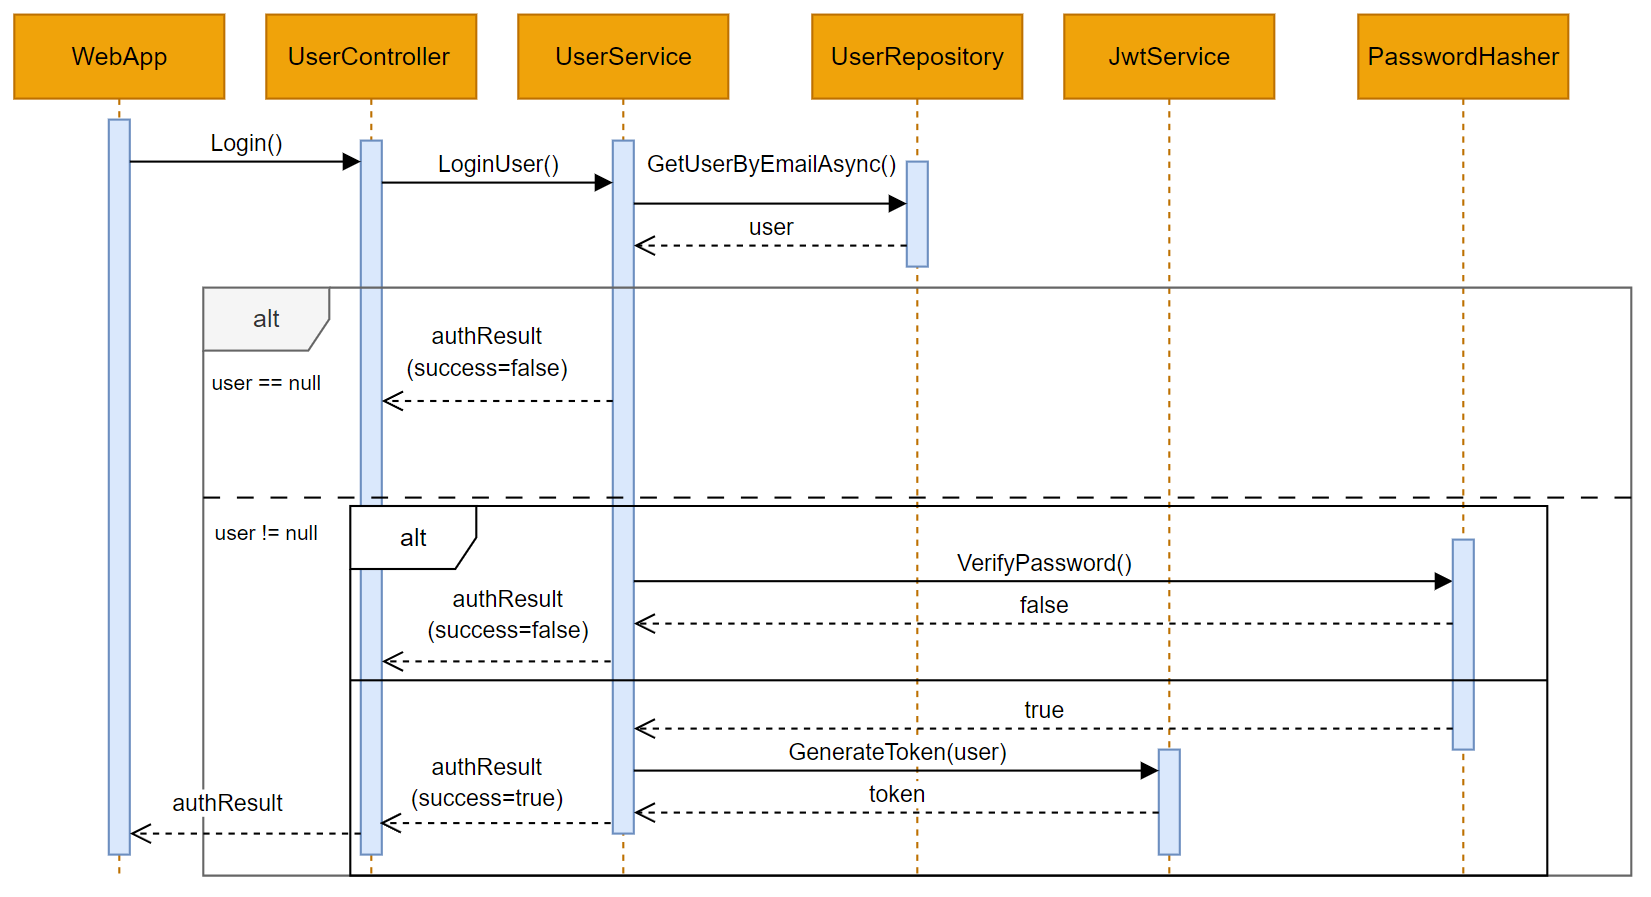
\includegraphics[width=0.9\textwidth]{images/login-flow.png}
    \caption{Login flow}
    \label{fig:login-flow}
\end{figure}